\chapter*{Wstęp}
\addcontentsline{toc}{chapter}{Wstęp}
\chapter{Wprowadzenie do problematyki}
\chapter{Technologie i narzędzia wykorzystywane w pracy}
W poniższym rozdziale zostały opisane wybrane technologie oraz narzędzia deweloperskie, wspomagające zapewnienie jakości kodu, wykorzystywane w trakcie implementacji systemu.
\section{Xamarin.Android}
\label{sec:xamAnd}
Xamarin.Android jest to platforma programistyczna stworzona z pomocą .NET Framework do tworzenia aplikacji na system operacyjny Android z wykorzystaniem natywnych metod SDK (\textit{Software Development Kit}) systemu Android. Z pomocą wyżej wymienionej platformy, aplikacje są tworzone w języku C\# (implementacja Xamarin.Android daje możliwość wykorzystywania specyficznych cech języka takich jak np. \textit{LINQ}). 

Kod źródłowy w C\#, w celu uzyskania natywnej aplikacji, jest kompilowany do IL (\textit{Common Intermediate Language}) z wykorzystaniem kompilatora MonoVM. MonoVM jest kompilatorem typu JIT (\textit{just-in-time compiler}). Program jest kompilowany w trakcie wykonywania, przed wykonaniem  danego fragmentu kodu, do kodu maszynowego.\cite{Part1–Un34:online}
Niewykorzystane klasy zawarte w frameworku są podczas kompilowania aplikacji usuwane z wykorzystaniem \textit{linkera}, w celu zmniejszenia rozmiaru aplikacji.\cite{Linkingo58:online}

Aplikacja działa obok natywnych aplikacjami (napisanymi w językach Java/Kotlin) w ART (\textit{Android Runtime} - środowisko uruchomieniowe systemu Android). Interakcje z wykorzystaniem natywnych typów odbywają się z pomocą JNI (\textit{Java Native Interface})\cite{Part1–Un34:online}

\section{Xamarin.iOS}
\label{sec:xamiOS}
Xamarin.iOS, podobnie jak Xamarin.Android, jest to platforma programistyczna stworzona z pomocą .NET Framework do tworzenia aplikacji na system operacyjny iOS. Wykorzystuje ona natywne metody SDK (\textit{Software Development Kit}) systemu iOS. Aplikacje są tworzone z wykorzystaniem języka C\#.

Kod źródłowy jest kompilowany z użyciem kompilacji AOT (\textit{Ahead-Of-Time}) do języka assemblera dla procesorów ARM. Do kodu jest dołączony framework .NET, którego nieużywane klasy są usuwane przy pomocy \textit{linkera} w celu zmniejszenia rozmiaru aplikacji.\cite{Part1–Un34:online}\cite{Linkingo42:online}

Jako, że firma Apple - twórca systemu iOS, nie pozwala na dynamiczne generowanie kodu w trakcie wykonywania programu, niektóre cechy języka C\# nie są dostępne dla twórcy aplikacji. (ograniczenia głównie dotyczą klas generycznych \cite{Limitati57:online} oraz mechanizmu refleksji \cite{Limitati74:online})
\section{ASP.NET Core}
\label{sec:aspCore}
\section{Entity Framework Core}
\label{sec:entityCore}
\section{Dapper}
\label{sec:dapper}
\section{MVVMCross}
\label{sec:mvvmCross}
MVVMCross jest to framework wspomagający tworzenie aplikacji według wzorca projektowego Model-View-ViewModel. MVVMCross jest przygotowany specjalnie pod kątem platformy Xamarin 
\section{AutoFac}
\label{sec:autoFac}
\section{Team Foundation Server}
\label{sec:team}
\section{HockeyApp}
\label{sec:hockeyapp}
\section{Microsoft Azure}
\label{sec:azure}
\chapter{Założenia projektowe}
W tym rozdziale zostaną omówione założenia projektowe systemu. Pierwszy podrozdział jest poświęcony opisowi przedmiotu pracy. W podrozdziałach drugim oraz trzecim zostały opisane wymagania odpowiednio funkcjonalne i niefunkcjonalne na system. Ostatni podrozdział jest to opis zaprojektowanej architektury systemu.
\section{Przedmiot pracy}
Przedmiotem pracy jest utworzenie aplikacji mobilnej na platformy Android oraz iOS, umożliwiającej rezerwację i zakup biletów kinowych w ramach sieci kin, wraz z towarzyszącą aplikacją serwerową. Aplikacja kliencka będzie utworzona w oparciu o platformę Xamarin [\ref{sec:xamAnd}][\ref{sec:xamiOS}], natomiast aplikacja serwerowa w oparciu o framework ASP.NET Core [\ref{sec:aspCore}]
\section{Wymagania funkcjonalne}
System powinien spełniać następujące wymagania funkcjonalne. Przy definiowaniu wymagań przyjęto następujących aktorów - Klient, Pracownik kina, Administrator systemu, System 
\begin{enumerate}
\item Jako Klient, chcę mieć możliwość stworzenia konta użytkownika na podstawie adresu e-mail, w celu zachowania preferencji użytkownika pomiędzy urządzeniami.
\item Jako Klient, chcę mieć możliwość stworzenia konta użytkownika z wykorzystaniem konta w jednym ze wspieranych portali społecznościowych (Facebook, Twitter, Google), w celu przyspieszenia procesu tworzenia konta.
\item Jako Klient, chcę mieć możliwość modyfikacji informacji o koncie użytkownika, w celu wygodnej aktualizacji danych.
\item Jako Klient, chcę mieć możliwość zresetowania hasła do konta użytkownika, w celu odzyskania dostępu do konta. 
\item Jako Klient, chcę mieć możliwość wyboru domyślnego kina, w celu łatwiejszego dostępu do aktualnego repertuaru.
\item Jako Klient, chcę mieć możliwość przeglądania aktualnego repertuaru w danym kinie, w celu zapoznania się z ofertą kina.
\item Jako Klient, chcę mieć możliwość przeglądania podstawowych informacji o filmie z repertuaru, w celu zapoznania się z krótkim opisem filmu. 
\item Jako Klient, chcę mieć możliwość złożenia rezerwacji biletu(ów) na wybrany seans w wybranym kinie, w celu późniejszej finalizacji zamówienia przed seansem.
\item System anuluje wszystkie niepotwierdzone rezerwacje 30 minut przed planowanym początkiem seansu. 
\item Jako Klient, chcę mieć możliwość zakupu biletu(ów) na wybrany seans w wybranym kinie, w celu braku konieczności kupna biletu w kasie stacjonarnej przed seansem.
\item Jako Klient, chcę mieć możliwość dokonania zapłaty za zakupione bilety za pośrednictwem zewnętrznego systemu płatności elektronicznych, w celu szybszej finalizacji zamówienia
\item Jako Klient, chcę mieć możliwość zwrotu zakupionych biletów do 3 godzin przed planowanym seansem, w celu odzyskania pieniędzy za niewykorzystane bilety.
\item Jako Klient, chcę mieć możliwość wyboru miejsc na podstawie widoku sali kinowej, w celu świadomego wyboru miejsca na sali kinowej.
\item Jako Klient, chcę mieć możliwość wyboru rodzaju biletu przy wyborze miejsc, w celu wyboru odpowiedniego rodzaju biletu (np. ulgowego dla osoby niepełnoletniej).
\item Jako Klient, chcę mieć możliwość przeglądania historii rezerwacji oraz zakupionych biletów, w celu   
\item Jako Klient, chcę mieć możliwość dokonania zakupu biletu(ów) bez potrzeby zakładania konta, w celu szybkiego złożenia pojedynczego zamówienia.
\item Jako Klient, chcę mieć możliwość dokonania rezerwacji biletu(ów) bez potrzeby zakładania konta, w celu szybkiego złożenia pojedynczej rezerwacji
\item Jako Klient, chcę mieć możliwość okazania biletu w formacie kodu QR, w celu ułatwienia weryfikacji biletu przy wejściu na salę kinową.
\item Jako Klient, chcę mieć możliwość okazania biletu pomimo braku połączenia z siecią Internet, w celu ograniczenia powszechnych problemów dotyczących połączenia internetowego przy okazywaniu biletu.\newline
\item Jako Pracownik kina, chcę mieć możliwość modyfikacji podstawowych danych o kinie, w celu aktualizacji danych.
\item Jako Pracownik kina, chcę mieć możliwość modyfikacji informacji o salach dostępnych w kinie, w celu aktualizacji ilości dostępnych miejsc na sali kinowej.
\item Jako Pracownik kina, chcę mieć możliwość modyfikacji repertuaru kina, w celu aktualizacji oferty kina.
\item Jako Pracownik kina, chcę mieć możliwość potwierdzenia rezerwacji klienta, w celu finalizacji zamówienia.
\item Jako Pracownik kina, chcę mieć możliwość anulowania rezerwacji klienta, w celu zapewnienia większego wyboru miejsc dla pozostałych Klientów.
\item Jako Pracownik kina, chcę mieć możliwość dokonania sprzedaży biletów klientom w kasie biletowej, w celu umożliwienia kupna biletów przez Klientów nie posiadających aplikacji.
\item Jako Administrator systemu, chcę mieć możliwość dodawania, modyfikowania i usuwania informacji o kinach należących do sieci kin, w celu weryfikacji danych o kinach.
\item Jako Administrator systemu, chcę mieć możliwość tworzenia oraz modyfikacji kont użytkowników oraz przydzielania im ról, w celu zarządzania dostępu użytkowników do systemu.
\end{enumerate}
Powyższa lista jest pełnym zbiorem wymagań, które powinny się znaleźć w ostatecznej wersji systemu. Prototyp systemu, będący celem pracy, będzie miał zaimplementowane wszystkie funkcjonalności dotyczące roli Klienta tj. wymagania od pierwszego do dziewiętnastego.
\section{Wymagania niefunkcjonalne}
Zbiór tych wymagań definiuje, jakie wymagania na system mają zostać spełnione, oprócz wymagań funkcjonalnych. Wymagania te głównie dotyczą wydajności, bezpieczeństwa i tym podobnych aspektów.
\begin{enumerate}
\item System powinien być dostępny bez przerwy. (Dostępność na poziomie 99,9\%)
\item System jest w stanie obsługiwać wiele jednocześnie podłączonych urządzeń.
\item Do poprawnego korzystania ze wszystkich funkcji oferowanych przez aplikację, wymagane jest stałe połączenie internetowe.
\item W celu zapewnienia odpowiedniego poziomu bezpieczeństwa, połączenie między serwerem i klientem ma być szyfrowane.
\item System ma wspierać również mechanizm sesji, jako dodatkowy mechanizm zabezpieczający połączenie.
\item Aplikacja kliencka powinna być dostępna na systemach Android (w wersji 4.4 i wyższej) oraz iOS (w wersji 8.0 i wyższej).
\item Aplikacja kliencka powinna zostać uruchomiona na urządzeniu mobilnym niezależnie od stanu połączenia internetowego.
\item Aplikacja serwerowa powinna móc być uruchomiona na serwerach z systemami rodziny Windows Server (wersja 2012 R2 i wyżej) oraz Linux

\end{enumerate}
\section{Opis podstawowej architektury systemu}
\subsection*{Architektura logiczna}
System będzie składał się z trzech aplikacji. 

\par Pierwszą z nich jest aplikacja serwerowa, realizowana w architekturze trójwarstwowej (podział na warstwę prezentacji, logiki biznesowej oraz dostępu do danych). Dzięki takiemu podziałowi, w którym wyższa warstwa nie wie o logice zawartej w niższej warstwie (\textit{black box}) zapewniamy m.in. dużą skalowalność rozwiązania (każdą warstwę możemy skalować według potrzeb) oraz ułatwione testowanie rozwiązania poprzez brak skomplikowanych zależności pomiędzy warstwami.

\par Operacje na bazie danych aplikacji będą wykonywane w warstwie dostępu do danych z częściowym wykorzystaniem podejścia CQRS (\textit{Command Query Responsibility Segregation}), które zapewni jeszcze lepszą skalowalność rozwiązania poprzez, przede wszystkim oddzielenie operacji zapisu danych od ich odczytu. Więcej szczegółów na temat podejścia CQRS oraz jego implementacji znajduje się w podrozdziale~\ref{sec:cqrs}

\par Pozostałą część systemu stanowią aplikacje mobilne działająca pod kontrolą systemu Android oraz iOS. Aplikacje te będą implementowane z wykorzystaniem platformy Xamarin. Dzięki temu możemy mówić o aplikacji wieloplatformowej, ponieważ większość kodu aplikacji (głównie chodzi tutaj o logikę zawartą w aplikacji) jest współdzielona. Aby umożliwić współdzielenie kodu, będzie zastosowany wzorzec architektoniczny Model-View-ViewModel. Dzięki temu wzorcowi dokonujemy separacji aplikacji na warstwy: widoku (View), logiki interfejsu (ViewModel) oraz modelu danych. Logika interfejsu oraz modelu danych są współdzielone, natomiast osobne widoki odpowiadają specyfice poszczególnych systemów. Wyseparowane warstwy sprawiają, że kod aplikacji jest o wiele bardziej testowalny oraz łatwiejszy w utrzymaniu. Do przechowywania danych lokalnych aplikacji posłuży baza danych SQLite.

\subsection*{Architektura fizyczna}
Aplikacja serwerowa zbudowana będzie w oparciu o framework ASP.NET Core. Będzie mieć ona możliwość pracowania na serwerach z systemami rodziny Windows Server oraz Linux. Wykorzystywany serwer WWW to, w zależności od wybranego systemu, IIS (\textit{Internet Information Services}) oraz Apache.

\par Aplikacja serwerowa będzie komunikować się z serwerem bazodanowym Microsoft SQL Server znajdującym się na osobnym serwerze (działającym pod kontrolą dystrybucji systemu Windows Server lub Linux), z wykorzystaniem protokołu TLS/SSL w celu zapewnienia odpowiedniego poziomu bezpieczeństwa.

\par W ramach realizowanego prototypu, serwery aplikacji oraz bazy danych będą hostowane na platformie obliczeniowej Microsoft Azure. 

\par Aplikacje klienckie działające na urządzeniach z systemami Android oraz iOS, będą komunikowały się z serwerem aplikacji, wykorzystując udostępnione przez aplikację \textit{RESTful API}. Formatem przesyłanych danych jest \textit{JSON}. Komunikacja odbywa się za pośrednictwem protokołu HTTPS (ruch jest szyfrowany).
\begin{figure}[h]
\centering
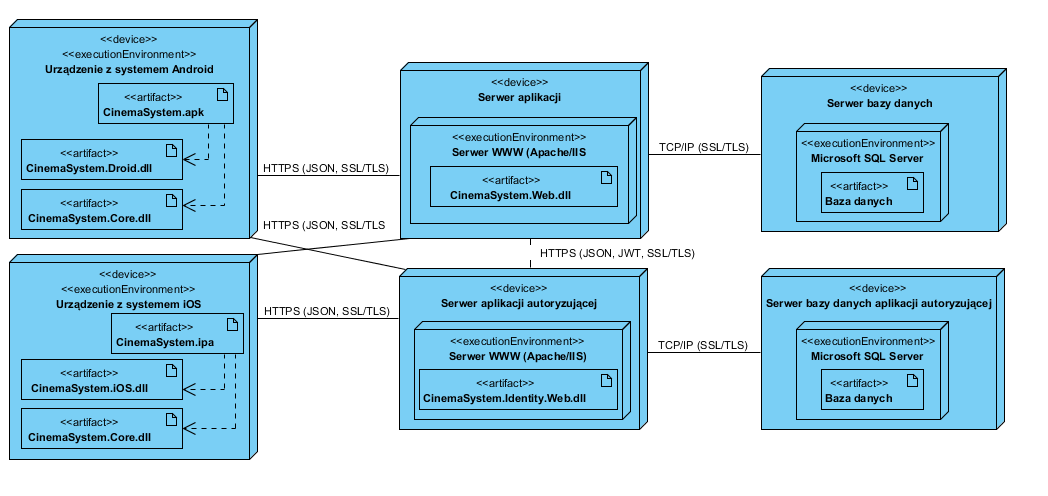
\includegraphics[width=1\textwidth]{img1}
\caption{Architektura fizyczna systemu}
\end{figure}
\chapter{Projekt aplikacji}
\section{Przypadki użycia}
\section{Interfejs}
\section{Diagram klas}
\addtocontents{toc}{\protect\newpage}
\chapter{Implementacja}
\section{DevOps}
\section{Autoryzacja użytkowników aplikacji}
\section{Synchronizacja danych offline-online}
\section{Bezpieczeństwo aplikacji}
\section{Implementacja wzorca CQRS}
\label{sec:cqrs}
\section{Testy interfejsu aplikacji}
\chapter{Podsumowanie}
\printbibliography[nottype=misc, title={Bibliografia},resetnumbers=true,heading=bibintoc]
\begin{refcontext}[labelprefix=L]
\printbibliography[type=misc, title={Netografia},resetnumbers=true,heading=bibintoc]
\end{refcontext}
\chapter*{Załączniki}
\addcontentsline{toc}{chapter}{Załączniki}
\section*{Spis tabel}
\addcontentsline{toc}{section}{Spis tabel}
\listoftables
\section*{Spis rysunków}
\addcontentsline{toc}{section}{Spis rysunków}
\listoffigures
\lstlistoflistings
\addcontentsline{toc}{section}{Spis listingów}
\section*{Instrukcja kompilacji i testowego uruchomienia aplikacji}
\addcontentsline{toc}{section}{Instrukcja kompilacji i testowego uruchomienia aplikacji}